% REV01 Tue 22 Jun 2021 17:30:50 WIB
% START Tue 04 May 2021 13:55:16 WIB

\chapter{A PIECE OF WORK}

Britannia, sitting meditating one fine day (perhaps in the attitude in
which she is presented on the copper coinage), discovers all of a sudden
that she wants Veneering in Parliament. It occurs to her that Veneering
is ‘a representative man’--which cannot in these times be doubted--and
that Her Majesty’s faithful Commons are incomplete without him. So,
Britannia mentions to a legal gentleman of her acquaintance that if
Veneering will ‘put down’ five thousand pounds, he may write a couple
of initial letters after his name at the extremely cheap rate of two
thousand five hundred per letter. It is clearly understood between
Britannia and the legal gentleman that nobody is to take up the five
thousand pounds, but that being put down they will disappear by magical
conjuration and enchantment.

The legal gentleman in Britannia’s confidence going straight from that
lady to Veneering, thus commissioned, Veneering declares himself highly
flattered, but requires breathing time to ascertain ‘whether his friends
will rally round him.’ Above all things, he says, it behoves him to be
clear, at a crisis of this importance, ‘whether his friends will rally
round him.’ The legal gentleman, in the interests of his client cannot
allow much time for this purpose, as the lady rather thinks she knows
somebody prepared to put down six thousand pounds; but he says he will
give Veneering four hours.

Veneering then says to Mrs Veneering, ‘We must work,’ and throws himself
into a Hansom cab. Mrs Veneering in the same moment relinquishes baby
to Nurse; presses her aquiline hands upon her brow, to arrange the
throbbing intellect within; orders out the carriage; and repeats in
a distracted and devoted manner, compounded of Ophelia and any
self-immolating female of antiquity you may prefer, ‘We must work.’

Veneering having instructed his driver to charge at the Public in the
streets, like the Life-Guards at Waterloo, is driven furiously to Duke
Street, Saint James’s. There, he finds Twemlow in his lodgings, fresh
from the hands of a secret artist who has been doing something to his
hair with yolks of eggs. The process requiring that Twemlow shall, for
two hours after the application, allow his hair to stick upright and dry
gradually, he is in an appropriate state for the receipt of startling
intelligence; looking equally like the Monument on Fish Street Hill, and
King Priam on a certain incendiary occasion not wholly unknown as a neat
point from the classics.

‘My dear Twemlow,’ says Veneering, grasping both his hands, ‘as the
dearest and oldest of my friends--’

(‘Then there can be no more doubt about it in future,’ thinks Twemlow,
‘and I AM!’)

‘--Are you of opinion that your cousin, Lord Snigsworth, would give his
name as a Member of my Committee? I don’t go so far as to ask for his
lordship; I only ask for his name. Do you think he would give me his
name?’

In sudden low spirits, Twemlow replies, ‘I don’t think he would.’

‘My political opinions,’ says Veneering, not previously aware of having
any, ‘are identical with those of Lord Snigsworth, and perhaps as a
matter of public feeling and public principle, Lord Snigsworth would
give me his name.’

‘It might be so,’ says Twemlow; ‘but--’ And perplexedly scratching his
head, forgetful of the yolks of eggs, is the more discomfited by being
reminded how stickey he is.

‘Between such old and intimate friends as ourselves,’ pursues Veneering,
‘there should in such a case be no reserve. Promise me that if I ask you
to do anything for me which you don’t like to do, or feel the slightest
difficulty in doing, you will freely tell me so.’

This, Twemlow is so kind as to promise, with every appearance of most
heartily intending to keep his word.

‘Would you have any objection to write down to Snigsworthy Park, and ask
this favour of Lord Snigsworth? Of course if it were granted I should
know that I owed it solely to you; while at the same time you would put
it to Lord Snigsworth entirely upon public grounds. Would you have any
objection?’

Says Twemlow, with his hand to his forehead, ‘You have exacted a promise
from me.’

‘I have, my dear Twemlow.’

‘And you expect me to keep it honourably.’

‘I do, my dear Twemlow.’

‘ON the whole, then;--observe me,’ urges Twemlow with great nicety, as
if; in the case of its having been off the whole, he would have done it
directly--‘ON the whole, I must beg you to excuse me from addressing any
communication to Lord Snigsworth.’

‘Bless you, bless you!’ says Veneering; horribly disappointed, but
grasping him by both hands again, in a particularly fervent manner.

It is not to be wondered at that poor Twemlow should decline to inflict
a letter on his noble cousin (who has gout in the temper), inasmuch
as his noble cousin, who allows him a small annuity on which he lives,
takes it out of him, as the phrase goes, in extreme severity; putting
him, when he visits at Snigsworthy Park, under a kind of martial law;
ordaining that he shall hang his hat on a particular peg, sit on a
particular chair, talk on particular subjects to particular people, and
perform particular exercises: such as sounding the praises of the Family
Varnish (not to say Pictures), and abstaining from the choicest of the
Family Wines unless expressly invited to partake.

‘One thing, however, I CAN do for you,’ says Twemlow; ‘and that is, work
for you.’

Veneering blesses him again.

‘I’ll go,’ says Twemlow, in a rising hurry of spirits, ‘to the
club;--let us see now; what o’clock is it?’

‘Twenty minutes to eleven.’

‘I’ll be,’ says Twemlow, ‘at the club by ten minutes to twelve, and I’ll
never leave it all day.’

Veneering feels that his friends are rallying round him, and says,
‘Thank you, thank you. I knew I could rely upon you. I said to Anastatia
before leaving home just now to come to you--of course the first friend
I have seen on a subject so momentous to me, my dear Twemlow--I said to
Anastatia, “We must work.”’

‘You were right, you were right,’ replies Twemlow. ‘Tell me. Is SHE
working?’

‘She is,’ says Veneering.

‘Good!’ cries Twemlow, polite little gentleman that he is. ‘A woman’s
tact is invaluable. To have the dear sex with us, is to have everything
with us.’

‘But you have not imparted to me,’ remarks Veneering, ‘what you think of
my entering the House of Commons?’

‘I think,’ rejoins Twemlow, feelingly, ‘that it is the best club in
London.’

Veneering again blesses him, plunges down stairs, rushes into his
Hansom, and directs the driver to be up and at the British Public, and
to charge into the City.

Meanwhile Twemlow, in an increasing hurry of spirits, gets his hair down
as well as he can--which is not very well; for, after these glutinous
applications it is restive, and has a surface on it somewhat in the
nature of pastry--and gets to the club by the appointed time. At the
club he promptly secures a large window, writing materials, and all
the newspapers, and establishes himself; immoveable, to be respectfully
contemplated by Pall Mall. Sometimes, when a man enters who nods to
him, Twemlow says, ‘Do you know Veneering?’ Man says, ‘No; member of
the club?’ Twemlow says, ‘Yes. Coming in for Pocket-Breaches.’ Man says,
‘Ah! Hope he may find it worth the money!’ yawns, and saunters out.
Towards six o’clock of the afternoon, Twemlow begins to persuade
himself that he is positively jaded with work, and thinks it much to be
regretted that he was not brought up as a Parliamentary agent.

From Twemlow’s, Veneering dashes at Podsnap’s place of business. Finds
Podsnap reading the paper, standing, and inclined to be oratorical
over the astonishing discovery he has made, that Italy is not England.
Respectfully entreats Podsnap’s pardon for stopping the flow of his
words of wisdom, and informs him what is in the wind. Tells Podsnap that
their political opinions are identical. Gives Podsnap to understand that
he, Veneering, formed his political opinions while sitting at the feet
of him, Podsnap. Seeks earnestly to know whether Podsnap ‘will rally
round him?’

Says Podsnap, something sternly, ‘Now, first of all, Veneering, do you
ask my advice?’

Veneering falters that as so old and so dear a friend--

‘Yes, yes, that’s all very well,’ says Podsnap; ‘but have you made up
your mind to take this borough of Pocket-Breaches on its own terms, or
do you ask my opinion whether you shall take it or leave it alone?’

Veneering repeats that his heart’s desire and his soul’s thirst are,
that Podsnap shall rally round him.

‘Now, I’ll be plain with you, Veneering,’ says Podsnap, knitting his
brows. ‘You will infer that I don’t care about Parliament, from the fact
of my not being there?’

Why, of course Veneering knows that! Of course Veneering knows that if
Podsnap chose to go there, he would be there, in a space of time that
might be stated by the light and thoughtless as a jiffy.

‘It is not worth my while,’ pursues Podsnap, becoming handsomely
mollified, ‘and it is the reverse of important to my position. But it
is not my wish to set myself up as law for another man, differently
situated. You think it IS worth YOUR while, and IS important to YOUR
position. Is that so?’

Always with the proviso that Podsnap will rally round him, Veneering
thinks it is so.

‘Then you don’t ask my advice,’ says Podsnap. ‘Good. Then I won’t give
it you. But you do ask my help. Good. Then I’ll work for you.’

Veneering instantly blesses him, and apprises him that Twemlow is
already working. Podsnap does not quite approve that anybody should
be already working--regarding it rather in the light of a liberty--but
tolerates Twemlow, and says he is a well-connected old female who will
do no harm.

‘I have nothing very particular to do to-day,’ adds Podsnap, ‘and I’ll
mix with some influential people. I had engaged myself to dinner, but
I’ll send Mrs Podsnap and get off going myself; and I’ll dine with you
at eight. It’s important we should report progress and compare notes.
Now, let me see. You ought to have a couple of active energetic fellows,
of gentlemanly manners, to go about.’

Veneering, after cogitation, thinks of Boots and Brewer.

‘Whom I have met at your house,’ says Podsnap. ‘Yes. They’ll do very
well. Let them each have a cab, and go about.’

Veneering immediately mentions what a blessing he feels it, to possess
a friend capable of such grand administrative suggestions, and really
is elated at this going about of Boots and Brewer, as an idea wearing
an electioneering aspect and looking desperately like business. Leaving
Podsnap, at a hand-gallop, he descends upon Boots and Brewer, who
enthusiastically rally round him by at once bolting off in cabs, taking
opposite directions. Then Veneering repairs to the legal gentleman in
Britannia’s confidence, and with him transacts some delicate affairs
of business, and issues an address to the independent electors of
Pocket-Breaches, announcing that he is coming among them for their
suffrages, as the mariner returns to the home of his early childhood: a
phrase which is none the worse for his never having been near the place
in his life, and not even now distinctly knowing where it is.

Mrs Veneering, during the same eventful hours, is not idle. No sooner
does the carriage turn out, all complete, than she turns into it, all
complete, and gives the word ‘To Lady Tippins’s.’ That charmer dwells
over a staymaker’s in the Belgravian Borders, with a life-size model
in the window on the ground floor of a distinguished beauty in a blue
petticoat, stay-lace in hand, looking over her shoulder at the town in
innocent surprise. As well she may, to find herself dressing under the
circumstances.

Lady Tippins at home? Lady Tippins at home, with the room darkened,
and her back (like the lady’s at the ground-floor window, though for a
different reason) cunningly turned towards the light. Lady Tippins is
so surprised by seeing her dear Mrs Veneering so early--in the middle of
the night, the pretty creature calls it--that her eyelids almost go up,
under the influence of that emotion.

To whom Mrs Veneering incoherently communicates, how that Veneering
has been offered Pocket-Breaches; how that it is the time for rallying
round; how that Veneering has said ‘We must work’; how that she is here,
as a wife and mother, to entreat Lady Tippins to work; how that the
carriage is at Lady Tippins’s disposal for purposes of work; how that
she, proprietress of said bran new elegant equipage, will return home on
foot--on bleeding feet if need be--to work (not specifying how), until
she drops by the side of baby’s crib.

‘My love,’ says Lady Tippins, ‘compose yourself; we’ll bring him in.’
And Lady Tippins really does work, and work the Veneering horses too;
for she clatters about town all day, calling upon everybody she knows,
and showing her entertaining powers and green fan to immense advantage,
by rattling on with, My dear soul, what do you think? What do
you suppose me to be? You’ll never guess. I’m pretending to be an
electioneering agent. And for what place of all places? Pocket-Breaches.
And why? Because the dearest friend I have in the world has bought it.
And who is the dearest friend I have in the world? A man of the name of
Veneering. Not omitting his wife, who is the other dearest friend I have
in the world; and I positively declare I forgot their baby, who is the
other. And we are carrying on this little farce to keep up appearances,
and isn’t it refreshing! Then, my precious child, the fun of it is that
nobody knows who these Veneerings are, and that they know nobody, and
that they have a house out of the Tales of the Genii, and give dinners
out of the Arabian Nights. Curious to see ‘em, my dear? Say you’ll know
‘em. Come and dine with ‘em. They shan’t bore you. Say who shall meet
you. We’ll make up a party of our own, and I’ll engage that they shall
not interfere with you for one single moment. You really ought to see
their gold and silver camels. I call their dinner-table, the Caravan.
Do come and dine with my Veneerings, my own Veneerings, my exclusive
property, the dearest friends I have in the world! And above all, my
dear, be sure you promise me your vote and interest and all sorts of
plumpers for Pocket-Breaches; for we couldn’t think of spending sixpence
on it, my love, and can only consent to be brought in by the spontaneous
thingummies of the incorruptible whatdoyoucallums.

Now, the point of view seized by the bewitching Tippins, that this same
working and rallying round is to keep up appearances, may have something
in it, but not all the truth. More is done, or considered to be
done--which does as well--by taking cabs, and ‘going about,’ than the
fair Tippins knew of. Many vast vague reputations have been made,
solely by taking cabs and going about. This particularly obtains in all
Parliamentary affairs. Whether the business in hand be to get a man in,
or get a man out, or get a man over, or promote a railway, or jockey
a railway, or what else, nothing is understood to be so effectual as
scouring nowhere in a violent hurry--in short, as taking cabs and going
about.

Probably because this reason is in the air, Twemlow, far from being
singular in his persuasion that he works like a Trojan, is capped by
Podsnap, who in his turn is capped by Boots and Brewer. At eight o’clock
when all these hard workers assemble to dine at Veneering’s, it is
understood that the cabs of Boots and Brewer mustn’t leave the door, but
that pails of water must be brought from the nearest baiting-place,
and cast over the horses’ legs on the very spot, lest Boots and Brewer
should have instant occasion to mount and away. Those fleet messengers
require the Analytical to see that their hats are deposited where they
can be laid hold of at an instant’s notice; and they dine (remarkably
well though) with the air of firemen in charge of an engine, expecting
intelligence of some tremendous conflagration.

Mrs Veneering faintly remarks, as dinner opens, that many such days
would be too much for her.

‘Many such days would be too much for all of us,’ says Podsnap; ‘but
we’ll bring him in!’

‘We’ll bring him in,’ says Lady Tippins, sportively waving her green
fan. ‘Veneering for ever!’

‘We’ll bring him in!’ says Twemlow.

‘We’ll bring him in!’ say Boots and Brewer.

Strictly speaking, it would be hard to show cause why they should not
bring him in, Pocket-Breaches having closed its little bargain, and
there being no opposition. However, it is agreed that they must ‘work’
to the last, and that if they did not work, something indefinite would
happen. It is likewise agreed that they are all so exhausted with the
work behind them, and need to be so fortified for the work before them,
as to require peculiar strengthening from Veneering’s cellar. Therefore,
the Analytical has orders to produce the cream of the cream of his
binns, and therefore it falls out that rallying becomes rather a trying
word for the occasion; Lady Tippins being observed gamely to inculcate
the necessity of rearing round their dear Veneering; Podsnap advocating
roaring round him; Boots and Brewer declaring their intention of reeling
round him; and Veneering thanking his devoted friends one and all, with
great emotion, for rarullarulling round him.

In these inspiring moments, Brewer strikes out an idea which is the
great hit of the day. He consults his watch, and says (like Guy Fawkes),
he’ll now go down to the House of Commons and see how things look.

‘I’ll keep about the lobby for an hour or so,’ says Brewer, with a
deeply mysterious countenance, ‘and if things look well, I won’t come
back, but will order my cab for nine in the morning.’

‘You couldn’t do better,’ says Podsnap.

Veneering expresses his inability ever to acknowledge this last service.
Tears stand in Mrs Veneering’s affectionate eyes. Boots shows envy,
loses ground, and is regarded as possessing a second-rate mind. They all
crowd to the door, to see Brewer off. Brewer says to his driver, ‘Now,
is your horse pretty fresh?’ eyeing the animal with critical scrutiny.
Driver says he’s as fresh as butter. ‘Put him along then,’ says Brewer;
‘House of Commons.’ Driver darts up, Brewer leaps in, they cheer him as
he departs, and Mr Podsnap says, ‘Mark my words, sir. That’s a man of
resource; that’s a man to make his way in life.’

When the time comes for Veneering to deliver a neat and appropriate
stammer to the men of Pocket-Breaches, only Podsnap and Twemlow
accompany him by railway to that sequestered spot. The legal gentleman
is at the Pocket-Breaches Branch Station, with an open carriage with a
printed bill ‘Veneering for ever’ stuck upon it, as if it were a wall;
and they gloriously proceed, amidst the grins of the populace, to a
feeble little town hall on crutches, with some onions and bootlaces
under it, which the legal gentleman says are a Market; and from the
front window of that edifice Veneering speaks to the listening earth.
In the moment of his taking his hat off, Podsnap, as per agreement made
with Mrs Veneering, telegraphs to that wife and mother, ‘He’s up.’

Veneering loses his way in the usual No Thoroughfares of speech, and
Podsnap and Twemlow say Hear hear! and sometimes, when he can’t by any
means back himself out of some very unlucky No Thoroughfare, ‘He-a-a-r
He-a-a-r!’ with an air of facetious conviction, as if the ingenuity of
the thing gave them a sensation of exquisite pleasure. But Veneering
makes two remarkably good points; so good, that they are supposed
to have been suggested to him by the legal gentleman in Britannia’s
confidence, while briefly conferring on the stairs.

Point the first is this. Veneering institutes an original comparison
between the country, and a ship; pointedly calling the ship, the Vessel
of the State, and the Minister the Man at the Helm. Veneering’s object
is to let Pocket-Breaches know that his friend on his right (Podsnap) is
a man of wealth. Consequently says he, ‘And, gentlemen, when the timbers
of the Vessel of the State are unsound and the Man at the Helm is
unskilful, would those great Marine Insurers, who rank among our
world-famed merchant-princes--would they insure her, gentlemen? Would
they underwrite her? Would they incur a risk in her? Would they have
confidence in her? Why, gentlemen, if I appealed to my honourable friend
upon my right, himself among the greatest and most respected of that
great and much respected class, he would answer No!’

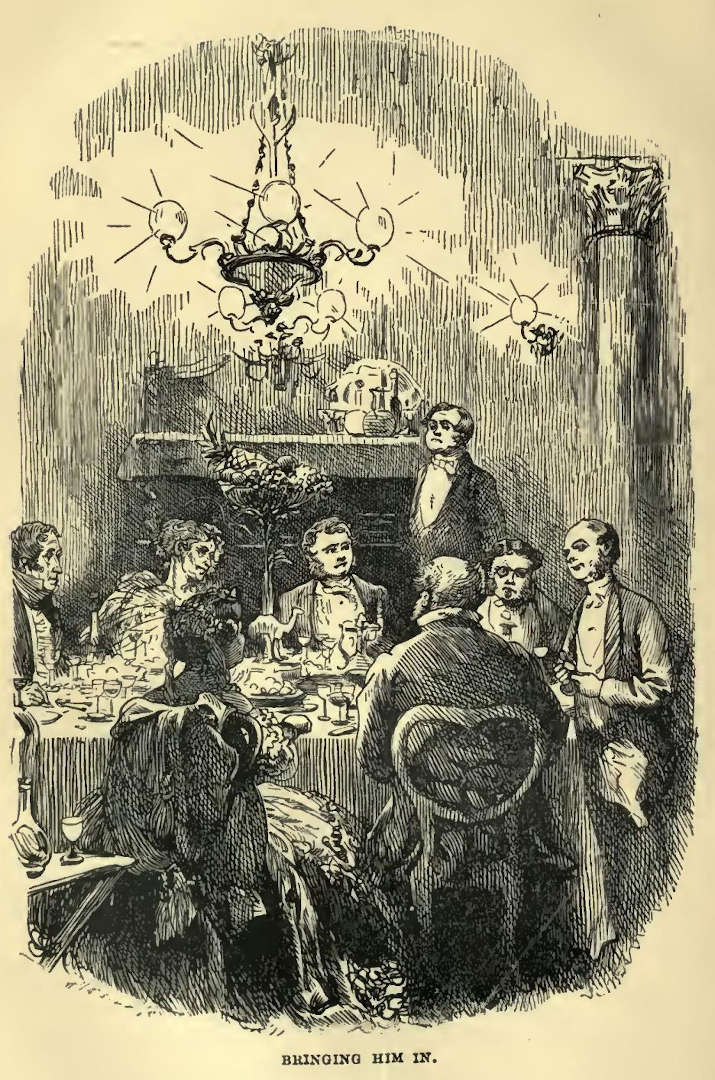
\includegraphics[scale=2.3]{02-03-01}

Point the second is this. The telling fact that Twemlow is related to
Lord Snigsworth, must be let off. Veneering supposes a state of public
affairs that probably never could by any possibility exist (though this
is not quite certain, in consequence of his picture being unintelligible
to himself and everybody else), and thus proceeds. ‘Why, gentlemen, if
I were to indicate such a programme to any class of society, I say it
would be received with derision, would be pointed at by the finger of
scorn. If I indicated such a programme to any worthy and intelligent
tradesman of your town--nay, I will here be personal, and say Our
town--what would he reply? He would reply, “Away with it!” That’s what
HE would reply, gentlemen. In his honest indignation he would reply,
“Away with it!” But suppose I mounted higher in the social scale.
Suppose I drew my arm through the arm of my respected friend upon my
left, and, walking with him through the ancestral woods of his family,
and under the spreading beeches of Snigsworthy Park, approached the
noble hall, crossed the courtyard, entered by the door, went up the
staircase, and, passing from room to room, found myself at last in
the august presence of my friend’s near kinsman, Lord Snigsworth. And
suppose I said to that venerable earl, “My Lord, I am here before your
lordship, presented by your lordship’s near kinsman, my friend upon my
left, to indicate that programme;” what would his lordship answer? Why,
he would answer, “Away with it!” That’s what he would answer, gentlemen.
“Away with it!” Unconsciously using, in his exalted sphere, the exact
language of the worthy and intelligent tradesman of our town, the near
and dear kinsman of my friend upon my left would answer in his wrath,
“Away with it!”’

Veneering finishes with this last success, and Mr Podsnap telegraphs to
Mrs Veneering, ‘He’s down.’

Then, dinner is had at the Hotel with the legal gentleman, and then
there are in due succession, nomination, and declaration. Finally Mr
Podsnap telegraphs to Mrs Veneering, ‘We have brought him in.’

Another gorgeous dinner awaits them on their return to the Veneering
halls, and Lady Tippins awaits them, and Boots and Brewer await
them. There is a modest assertion on everybody’s part that everybody
single-handed ‘brought him in’; but in the main it is conceded by all,
that that stroke of business on Brewer’s part, in going down to the
house that night to see how things looked, was the master-stroke.

A touching little incident is related by Mrs Veneering, in the course of
the evening. Mrs Veneering is habitually disposed to be tearful, and
has an extra disposition that way after her late excitement. Previous
to withdrawing from the dinner-table with Lady Tippins, she says, in a
pathetic and physically weak manner:

‘You will all think it foolish of me, I know, but I must mention it. As
I sat by Baby’s crib, on the night before the election, Baby was very
uneasy in her sleep.’

The Analytical chemist, who is gloomily looking on, has diabolical
impulses to suggest ‘Wind’ and throw up his situation; but represses
them.

‘After an interval almost convulsive, Baby curled her little hands in
one another and smiled.’

Mrs Veneering stopping here, Mr Podsnap deems it incumbent on him to
say: ‘I wonder why!’

‘Could it be, I asked myself,’ says Mrs Veneering, looking about her for
her pocket-handkerchief, ‘that the Fairies were telling Baby that her
papa would shortly be an M. P.?’

So overcome by the sentiment is Mrs Veneering, that they all get up
to make a clear stage for Veneering, who goes round the table to the
rescue, and bears her out backward, with her feet impressively scraping
the carpet: after remarking that her work has been too much for her
strength. Whether the fairies made any mention of the five thousand
pounds, and it disagreed with Baby, is not speculated upon.

Poor little Twemlow, quite done up, is touched, and still continues
touched after he is safely housed over the livery-stable yard in
Duke Street, Saint James’s. But there, upon his sofa, a tremendous
consideration breaks in upon the mild gentleman, putting all softer
considerations to the rout.

‘Gracious heavens! Now I have time to think of it, he never saw one of
his constituents in all his days, until we saw them together!’

After having paced the room in distress of mind, with his hand to his
forehead, the innocent Twemlow returns to his sofa and moans:

‘I shall either go distracted, or die, of this man. He comes upon me too
late in life. I am not strong enough to bear him!’



